\section{Evaluation}

We evaluate R2CC extensively on a real testbed and large-scale simulations. We find that:
\begin{packeditemize}
    \item R2CC achieves less than 1.1\% overhead on training and less than 3\% on inference when failure happens, reducing overhead by up to 92\% compared to training baselines and up to 98\% compared to inference baselines (§\ref{exp:training}, §\ref{exp:inference}).
    \item R2CC demonstrates robust scalability, incurring only 4.3\% overhead with 10 concurrent failures across a simulated 512-GPU cluster (§\ref{exp:training}).
    \item R2CC maintains up to 93\% of baseline throughput for collective operations during failures (§\ref{exp:overhead}).
\end{packeditemize}

\subsection{Methodology}
\label{sec:setup}
\textbf{Testbed.} Our physical testbed consists of four server nodes interconnected via InfiniBand fabric. Each node is equipped with 8 NVIDIA H100-80GB SXM5 GPUs, and 8 ConnectX-7 400Gbps InfiniBand NICs\footnote{InfiniBand SHARP is not enabled on our shared testbed; we discuss R2CC with SHARP in Appendix~\ref{app:discussion}.}. The intra-node GPUs support NVLink 4.0, providing 900GB/s bidirectional bandwidth. We use all four nodes for data-parallel training and the microbenchmarks, and two nodes for the TP=8, PP=2 training and inference runs. This configuration covers typical distributed training paradigms, allowing us to evaluate R2CC under realistic network conditions and failure scenarios.

For simulation experiments, we use SimAI~\cite{wang2025simai}, a high-fidelity ML training simulator that provides end-to-end training performance estimation, packet-level network modeling, and precise collective communication timing. SimAI has been validated against real-system performance and adopted in recent studies~\cite{qin2025phantora,gui2025accelerating,huang2025netzip}. We configure SimAI with NVIDIA's Spectrum-X RoCE-v2 rail-optimized topology, with each simulated server equipped with eight NVIDIA A100 GPUs and eight 200\,Gbps NICs. To evaluate the scalability of R2CC, we simulate clusters of 32 to 1024 GPUs, beyond the scale of our physical testbed.

\smallskip\noindent\textbf{Baselines.} For training experiments, we compile PyTorch v2.10.0 with NCCL v2.23.4 and with R2CC, and compare with these approaches: (1) {\bf Vanilla NCCL}~\cite{NCCL}, which crashes on NIC failure; (2) {\bf AdapCC}~\cite{zhao2024adapcc}, which excludes failed GPUs; (3) {\bf SHIFT}~\cite{shift}, which tolerates NIC failures by transparently failing over RDMA traffic to another intra-host NIC. (4) {\bf ICCL}~\cite{chen2025efficient}, which tolerates NIC port failures by always switching communication to a backup queue pair.

For inference experiments, we compile NCCL v2.23.4 and R2CC and build vLLM v1 on top. Because NCCL lacks fault tolerance, we implement two standard mitigation strategies: (1) {\bf Restart Server}, which incurs a measured 35-second restart delay, and (2) {\bf Reroute Request}, which redirects affected queries to an alternative server that must absorb the doubled load. We also evaluate {\bf DéjàVu}~\cite{ICML2024}, a fault-tolerant inference framework with KV-cache replication, compiled with both vanilla NCCL and R2CC to isolate R2CC's contribution.

For microbenchmarks, we use NCCL-tests v2.17.1 on all four nodes to compare vanilla NCCL and R2CC for collective and point-to-point operations under normal and single-NIC failure conditions.

\subsection{Training Resilience}
\label{exp:training}

\begin{figure}[t]
  \centering

  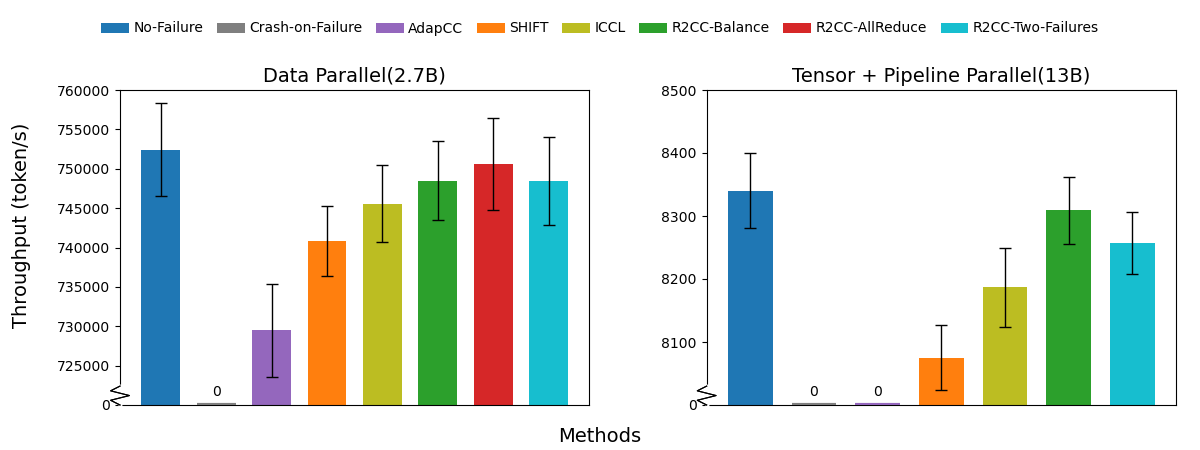
\includegraphics[width=\columnwidth]{figs/section8/Megatron_DP_TP_throughput_2.7B_13B_multif_new.png}
  \vspace{-5mm}
  \tightcaption{Megatron Training Performance Evaluation}
  \label{fig:megatron}
  \vspace{-3mm}
\end{figure}

In this section, we demonstrate R2CC's effectiveness in maintaining training continuity when failures occur. We use Megatron-LM\cite{narayanan2021efficient} as our training benchmark to compare against baselines.

\smallskip\noindent\textbf{Physical testbed evaluation.}
We measure token-per-second training throughput (Figure \ref{fig:megatron}) and overhead relative to a no-failure baseline for GPT-3 2.7B and 13B models under two multi-node configurations:
(1) DP=32 on the 2.7B model, where inter-node all-reduce dominates;
(2) TP=8, PP=2 on the 13B model, where pipeline stages span nodes and induce point-to-point activations.

Under DP=32, vanilla NCCL fails completely. Among fault-tolerant methods, R2CC-AllReduce achieves 750,627 tokens/s, just 0.24\% overhead vs.\ the no-failure throughput of 752,405 tokens/s. R2CC-Balance incurs 0.43\%, SHIFT and ICCL incur 1.57\% and 0.92\% respectively. AdapCC is the slowest (3.14\%) due to reduced compute capacity.

For TP=8, PP=2 on the 13B model, R2CC-Balance performs best, with only 0.38\% overhead (8,309 vs. 8,340 tokens/s). SHIFT and ICCL incur 3.28\% and 1.88\% respectively. AdapCC cannot operate in this setting (0 tokens/s) because removing a rank violates tensor/pipeline partitioning constraints.

AdapCC can exclude failed GPUs only if the failure occurs before a collective begins, so mid-operation faults still crash the job and excluded GPUs cause gradient loss. R2CC instead reroutes traffic through healthy NICs mid-operation and preserves full-rank, lossless execution.

To assess resilience under more severe conditions, we inject two simultaneous NIC failures on one node. In DP=32, R2CC-Two-Failures sustains 749,134 tokens/s (0.44\% overhead). In TP=8, PP=2, it delivers 8,257 tokens/s (1.01\% overhead). In both cases, training proceeds with near-baseline efficiency, demonstrating R2CC's robustness to multiple failures.

\smallskip\noindent\textbf{Training quality.} On a separate three-server testbed with six NVIDIA Tesla V100S GPUs, we train GPT-2~\cite{radford2019language} (124M) through a NIC-port failure and compare it with NCCL runs. Failure-free R2CC matches NCCL bit for bit, and the collective repaired by HotRepair yields a bit-identical gradient. The degraded schedules change only the order in which gradients are reduced, and since floating-point addition is not associative, this introduces rounding-level deviations: the per-update training loss differs by at most $2.4\times10^{-3}$ nats/token and final test perplexity by at most 0.023\% (Appendix~\ref{app:quality}).

\begin{figure}[t]
    \centering

    \begin{subfigure}[b]{0.48\columnwidth}
        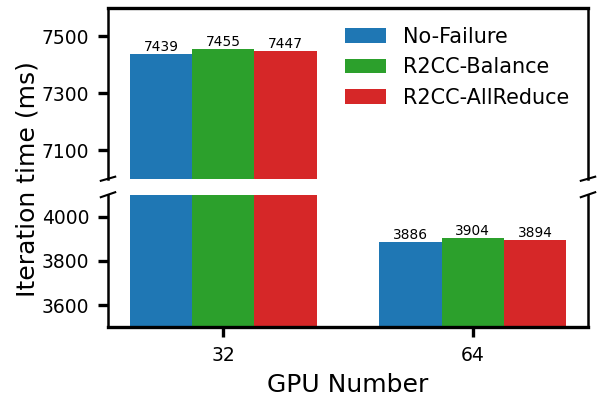
\includegraphics[width=\textwidth]{figs/small.png}
        \caption{Small Scale Training.}
        \label{fig:training-small}
    \end{subfigure}
    \hfill
    \begin{subfigure}[b]{0.48\columnwidth}
        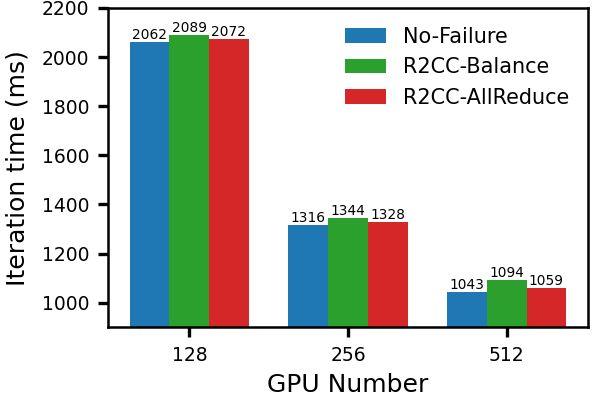
\includegraphics[width=\textwidth]{figs/large.png}
        \caption{Large Scale Training.}
        \label{fig:training-large}
    \end{subfigure}

    \vskip\baselineskip

    \begin{subfigure}[b]{0.48\columnwidth}
        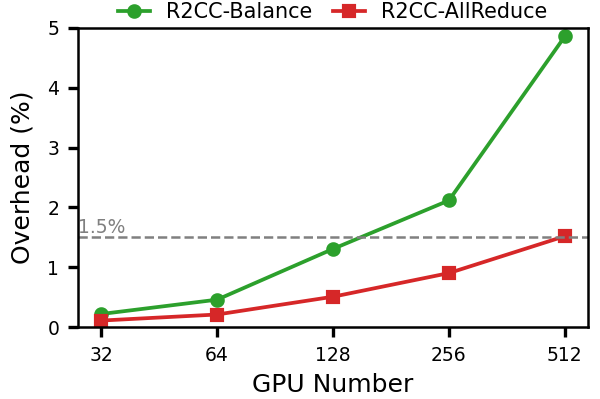
\includegraphics[width=\textwidth]{figs/ratio.png}
        \caption{Strategies Overhead.}
        \label{fig:training-e2eoverhead}
    \end{subfigure}
    \hfill
    \begin{subfigure}[b]{0.48\columnwidth}
        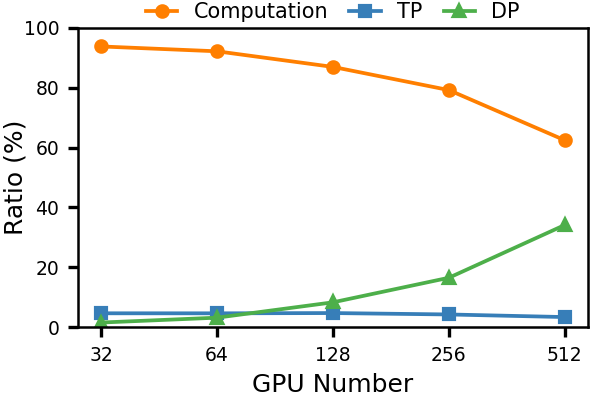
\includegraphics[width=\textwidth]{figs/e2e/training/compose.png}
        \caption{Time Composition.}
        \label{fig:training-e2eratio}
    \end{subfigure}

    \tightcaption{Simulated 7B model training on 4--64 8$\times$A100 servers.}
    \label{fig:training-all}
\end{figure}

\smallskip\noindent\textbf{Large scale training simulation under failures.}
For a single failure, we use SimAI to simulate a 7B-parameter model with global batch size 512, from 4 to 64 servers each with 8 GPUs. Within each server, GPUs are partitioned into two TP groups. Figure~\ref{fig:training-e2eoverhead} shows that R2CC-AllReduce consistently maintains an overhead of less than 1.5\% despite a 12.5\% bandwidth loss, significantly outperforming the R2CC-Balance strategy, which sees overhead rise to 5\% at larger scales. Overheads increase as the number of GPUs increases, because communication ratio increases when per GPU computation batch decreases, as shown in Figure~\ref{fig:training-e2eratio}.
Figure~\ref{fig:extra_training_time} shows pre-training a 175B-parameter model with 1,024 GPUs (TP=8, PP=8, DP=16) and RLHF fine-tuning with DeepSpeed-Chat's RLHF~\cite{yao2023deepspeedchateasyfastaffordable} on 64 GPUs (TP=8, PP=1, DP=8) with Fully Sharded Data Parallelism (FSDP). In this production scenario, R2CC proved vastly superior to the AdapCC framework reducing failure-induced training time by approximately 54$\times$ and 15$\times$, respectively.

We also extend our evaluation to scenarios with multiple concurrent failures. Unlike single-failure cases where the impact is deterministic, the performance degradation in multi-failure scenarios depends heavily on the spatial distribution of faults. We randomly inject $k$ failures across 64 servers (512 GPUs), varying $k$ from 1 to 10. We conduct a Monte Carlo simulation with 50 random failure patterns for each $k$. Figure~\ref{fig:training_multi_failures} shows the average iteration time overhead for the 7B model training as the number of failures increases. R2CC demonstrates exceptional resilience: the overhead grows sub-linearly from 1.5\% with a single failure to only 4.3\% with 10 concurrent failures. When multiple failures concentrate on a single server, that server becomes a bandwidth bottleneck; when failures scatter across the cluster, the impact is amortized and no single server dominates the critical path. This confirms that R2CC's load-balancing and algorithmic optimizations effectively bound performance degradation even under severe failure scenarios.

\begin{figure}[t]
    \centering
    \begin{minipage}[t]{0.49\linewidth}
        \centering
        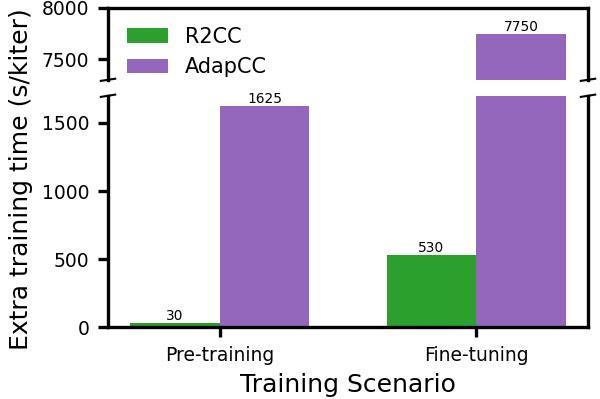
\includegraphics[width=\linewidth]{figs/extra-training-time.png}
        \vspace{-10pt}
        \tightcaption{Extra training time in R2CC vs. AdapCC.}
        \label{fig:extra_training_time}
    \end{minipage}
    \hfill
    \begin{minipage}[t]{0.49\linewidth}
        \centering
        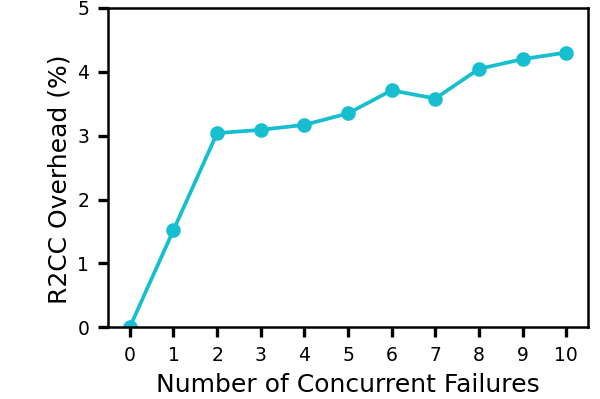
\includegraphics[width=\linewidth]{figs/multi_failures.png}
        \vspace{-10pt}
        \tightcaption{Multi-failure training overhead.}
        \label{fig:training_multi_failures}
    \end{minipage}
\end{figure}
\subsection{Inference Resilience}\label{exp:inference}

\begin{figure}
    \centering
    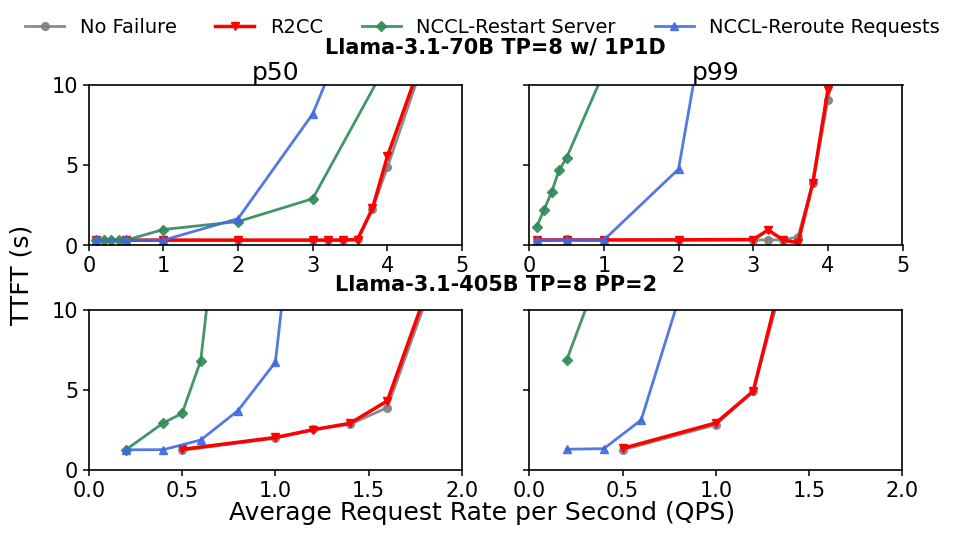
\includegraphics[width=1\linewidth]{figs/new-inference.png}
    \vspace{-10pt}
    \tightcaption{p50/p99 TTFT vs QPS under NIC failure for vLLM}
    \label{fig:vllm_results}
    \vspace{-3mm}
\end{figure}

\begin{figure}[t]
    \centering
    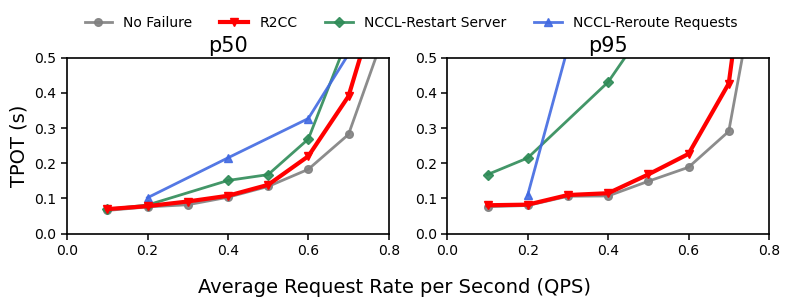
\includegraphics[width=1\linewidth]{figs/new-TPOT.png}
    \vspace{-10pt}
    \tightcaption{
    p50/p95 TPOT under NIC failure for serving Llama-3.1-405B with TP = 8, PP = 2.}
    \label{fig:tpot}
    \vspace{-3mm}
\end{figure}

In this section, we demonstrate how R2CC leverages network redundancy to significantly benefit end-to-end inference performance
when network failures occur. We evaluate R2CC using vLLM\cite{kwon2023efficient}, a widely adopted production inference framework, and compare it against two strategies relied upon by systems lacking transport-layer resilience: restarting the failed service and rerouting the requests to another server. Additionally, we integrate R2CC into DéjàVu\cite{ICML2024}, an existing fault-tolerant inference framework, to compare R2CC with its application-side fault tolerance.

\paragraph{vLLM Inference Performance.}
We use the vLLM v1 engine and focus on two multi-node configurations that exercise inter-node communication:
(i) tensor-parallelism with pipeline parallelism (TP=8, PP=2), and
(ii) TP=8 with prefill–decode (PD) disaggregation setting, which separates the compute-intensive prefill phase from the memory-intensive decode phase across different nodes.
These are vLLM configurations that require inter-node communication rather than being confined to a single node.

For each setup, we generate requests at fixed arrival rates. We measure different metrics tailored to each configuration's characteristics. For PD disaggregation, inter-node network failures primarily impact the prefill phase, making time-to-first-token (TTFT) our key metric since decoding proceeds without inter-node communication after the prefill node finishes transferring the KV cache. The pipeline-parallel configuration requires inter-node communication for every token generation, so we track both TTFT and time-per-output-token (TPOT) to capture the full performance impact.

Our experiments simulate inference patterns using 2000-token synthetic prompts, allowing models to generate outputs until reaching EOS or 256 tokens. Each 100-second experiment injects a single NIC failure at the midpoint (t=50s) to observe both transient and steady-state effects.

\paragraph{End-to-end latency (TTFT).}
Fig.~\ref{fig:vllm_results} plots TTFT as a function of the offered load for Llama-3.1-70B and 3.1-405B under different failure-handling strategies.
R2CC almost overlaps with the no-failure curve across models and percentiles (p50/p99),
indicating near-zero overhead under a NIC failure: before saturation, the TTFT overhead is within $\approx$0--0.6\% for the 70B model and 0.3--3\% for the 405B model.
Under a TTFT SLO of 5\,s, R2CC sustains up to 1.2--8.7$\times$ higher throughput than service restart and 1.6--1.9$\times$ higher throughput than request rerouting, while retaining $\approx$99–100\% of the no-failure capacity.

\paragraph{Streaming latency (TPOT).}
Fig.~\ref{fig:tpot} reports time per output token (TPOT) for the Llama-3.1-405B TP+PP configuration.
R2CC again closely tracks the no-failure baseline: both p50 and p95 TPOT increase smoothly with QPS and remain low until the system saturates, showing that R2CC preserves the streaming rate of generated tokens.
Before saturation, the TPOT overhead is within 3\%.
Under a p95 TPOT SLO of 0.4 s, R2CC sustains $\approx$1.9× and $\approx$2.6× higher throughput than the restart and rerouting strategies, respectively, while remaining within about 5\% of the no-failure capacity.

Appendix~\ref{multi-failure-inference} presents results under multiple failures.

\paragraph{Performance Comparison vs. DéjàVu.}
We follow DéjàVu's evaluation methodology and keep the application stack unchanged, varying only the communication layer. Using two workers with TP8 and PP2 parallelism, we evaluate the same models—OPT-66B and BLOOM-176B—under homogeneous requests (500-token prompt, 1500-token generation) and inject failure at decode step 800. As in their study, we report single-request cumulative latency. For comparison, we compile DéjàVu in two forms: (i) its original NCCL-based build and (ii) a version where NCCL is replaced by R2CC. This setup also demonstrates that R2CC integrates seamlessly without requiring any application-level modifications.

\begin{figure}[t]
    \centering
    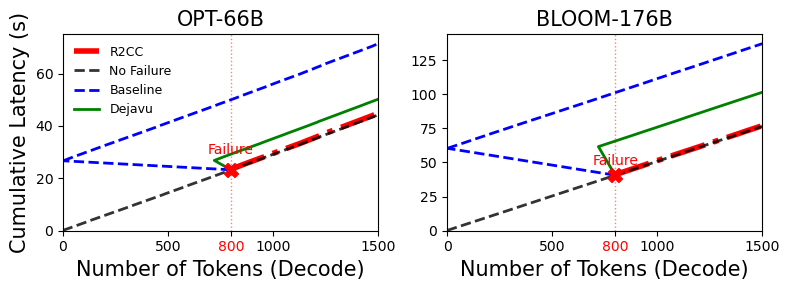
\includegraphics[width=1\linewidth]{figs/experiments/dejavu2.png}
    \vspace{-10pt}
    \tightcaption{Inference performance under failure compared to DéjàVu and non-fault-tolerant baseline.}
    \label{fig:dejavu}
\end{figure}

For DéjàVu and the non-fault-tolerant baseline, recovery is dominated by worker restart and reconnection delays. As shown in Figure~\ref{fig:dejavu}, the non-fault-tolerant baseline experiences severe latency inflation: $1.62\times$ for OPT-66B and 1.79$\times$ for BLOOM-176B—due to full request reprocessing. DéjàVu reduces this via neighbor KV-cache replication but still incurs a 14–33\% penalty (1.14$\times$–1.33$\times$) from bandwidth-heavy state reconstruction and added memory overhead. In contrast, R2CC's transparent connection migration avoids both restart and reconstruction, sustaining service with only 0.71–1.58\% overhead.
R2CC reduces recovery overhead by about 89--95\% for OPT-66B and 95--98\% for BLOOM-176B. Relative to the non-fault-tolerant baseline, the reduction is about 97--99\% for both models.

\subsection{Microbenchmarks}\label{exp:overhead}
\label{sec:microbenchmark}

We evaluate R2CC's primitive communication performance using NCCL-tests on four nodes of our physical testbed, measuring communication operations bus bandwidth across message sizes from 8B to 16GB under a failure scenario.

\paragraph{AllReduce Performance.}
Figure~\ref{fig:allreduce-h100} compares four configurations: vanilla NCCL with no failure, R2CC-HotRepair, R2CC-Balance, and R2CC-AllReduce. We also run the full R2CC pipeline with failures injected and fixed to measure R2CC's behavior with failover and restoration.

Without failure, vanilla NCCL achieves up to 393 GB/s for large messages. When a NIC fails (12.5\% total bandwidth loss), the R2CC-HotRepair approach suffers approximately 50\% throughput loss for large messages, as expected from the single-NIC bottleneck on the affected node.

R2CC's two strategies exhibit complementary strengths. For small messages ($<$32MB), R2CC-Balance achieves significantly lower latency, maintaining 88--96\% of normal throughput while R2CC-AllReduce ranges 73--94\% due to its data dependency coordination overhead. For medium messages (32MB--256MB), both strategies perform similarly at 88--96\% of normal throughput. For large messages ($\geq$512MB), R2CC-AllReduce achieves superior performance, around 88--93\% of normal throughput compared to Balance's 86--88\%, by reducing the data volume that the bandwidth-constrained node must transmit. These large-message ratios match the closed-form predictions from Section~\ref{sec:single-failure}: at $n = 4$ and $X = 1/8$, Balance throughput is expected to be $(1-X) = 87.5\%$ of baseline and R2CC-AllReduce throughput $\frac{2(n-1)(1-X)}{2(n-1)(1-X)+nX} = 91.3\%$, both falling within the measured ranges.

In practice, R2CC leverages an $\alpha$-$\beta$ performance model, using machine-specific link latency ($\alpha$) and bandwidth ($\beta$) parameters provided by NCCL along with the operation's data size, to dynamically select the optimal strategy at runtime. This approach ensures that the crossover point adapts to different hardware configurations and message sizes, rather than relying on a fixed threshold.

We evaluate the full R2CC pipeline from HotRepair to restore with a 1~GB message size nccl-tests AllReduce benchmark and compare its performance across different policies. As illustrated in Figure~\ref{fig:tiaolaitiaoqu}, we inject a network failure midway through iteration 5 and restore the connection at iteration 11. R2CC immediately repairs the in-flight collectives when the failure occurs, which causes a temporary dip in the average bandwidth for iteration 5. Starting from iteration 6, R2CC adapts to the optimal R2CC-AllReduce strategy, continuing the operation with only a 6.9\% overhead compared to the failure-free baseline. Once the network is restored at iteration 11, R2CC automatically reverts to the original AllReduce schedule. We also evaluate a case where a NIC fails mid-training between two scheduled checkpoints in Appendix~\ref{appendix:checkpoint}.

\paragraph{More results on other collectives.} Beyond AllReduce, we evaluate R2CC-Balance on AllGather, ReduceScatter, and point-to-point (SendRecv) operations. Appendix~\ref{appendix:collectives} shows that R2CC-Balance consistently maintains 85-89\% of normal throughput across all three operations.

\begin{figure}[t]
    \centering
    \begin{minipage}[t]{0.48\linewidth}
        \centering
        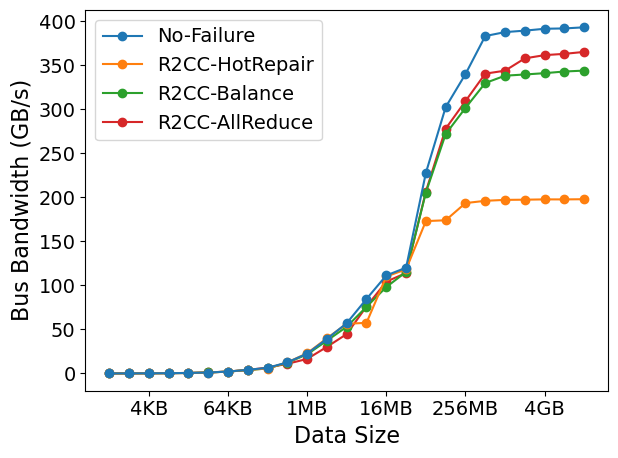
\includegraphics[width=1\textwidth]{figs/section8/all_reduce_v1.png}
        \vspace{-10pt}
        \tightcaption{AllReduce bandwidth vs. different message sizes using different R2CC configurations.}
        \label{fig:allreduce-h100}
    \end{minipage}
    \hfill
    \begin{minipage}[t]{0.48\linewidth}
        \centering
        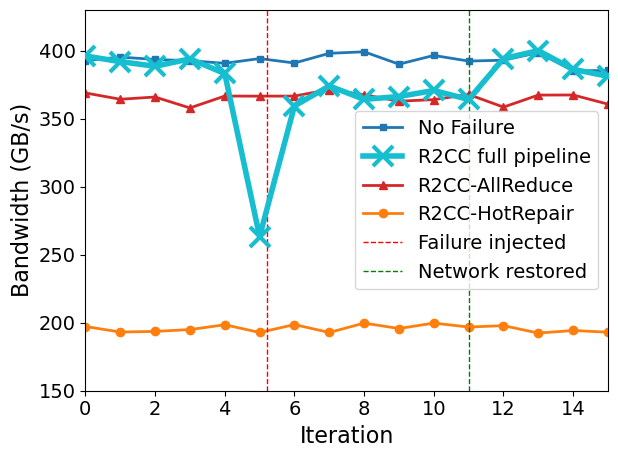
\includegraphics[width=\linewidth]{figs/tiaolaitiaoqu.png}
        \vspace{-10pt}
        \tightcaption{AllReduce bandwidth at message size 1GB with R2CC pipeline for failover and restore.}
        \label{fig:tiaolaitiaoqu}
    \end{minipage}
\end{figure}
